\documentclass[xcolor=x11names, svgnames, rgb]{beamer}

\setbeamertemplate{navigation symbols}{}
\setbeamercolor{block title}{bg=blue!40}
\setbeamercolor{block body}{bg=blue!20}

%% Beamer Layout %%%%%%%%%%%%%%%%%%%%%%%%%%%%%%%%%%
\useoutertheme[subsection=false,shadow]{miniframes}
\useinnertheme{default}
\usefonttheme{serif}
\usepackage{palatino}
\setbeamerfont{title like}{shape=\scshape}
\setbeamerfont{frametitle}{shape=\scshape}
\setbeamercolor*{lower separation line head}{bg=DeepSkyBlue4}
\setbeamercolor*{normal text}{fg=black,bg=white}
\setbeamercolor*{alerted text}{fg=red}
\setbeamercolor*{example text}{fg=black}
\setbeamercolor*{structure}{fg=black}
\setbeamercolor*{palette tertiary}{fg=black,bg=black!10}
\setbeamercolor*{palette quaternary}{fg=black,bg=black!10}
%% END Beamer Layout %%%%%%%%%%%%%%%%%%%%%%%%%%%%%%%%%%%%%%%%%%%%
\usepackage{graphicx}
\usepackage{algpseudocode}
\usepackage{soul}

\usepackage{mathtools}
\newcommand{\defeq}{\vcentcolon=}
\DeclarePairedDelimiter{\paren}{(}{)}

\newcommand{\dec}{\operatorname{dec}}
\newcommand{\poly}{\operatorname{poly}}
\newcommand{\polylog}{\operatorname{polylog}}
\newcommand{\github}{\url{github.com/awestover/Parallel-Partition}}
\newcommand{\defn}[1]       {{\textit{\textbf{\boldmath #1}}}}
\newcommand{\paragraph}[1]{\vspace{0.09in}\noindent{\bf \boldmath #1.}} 
\usepackage{amsmath}
\def\E{\operatorname{\mathbb{E}}}
\usepackage{amssymb}
\usepackage{amsthm}

\newtheorem{proposition}{Proposition}
\newtheorem{defin}{Definition}

\usepackage{hyperref}

\usepackage{tikz,pgfplots}
\usepackage{etoolbox}
%% This makes the colors annoyingly bright, but at least they're easy to distinguish.
\pgfplotsset{
  every  tick/.style={red,}, minor x tick num=1,
  cycle list={teal,every mark/.append style={fill=teal!80!black},mark=*\\%
orange,every mark/.append style={fill=orange!80!black},mark=square*\\%
cyan!60!black,every mark/.append style={fill=cyan!80!black},mark=otimes*\\%
red!70!white,mark=star\\%
lime!80!black,every mark/.append style={fill=lime},mark=diamond*\\%
red,densely dashed,every mark/.append style={solid,fill=red!80!black},mark=*\\%
yellow!60!black,densely dashed,
every mark/.append style={solid,fill=yellow!80!black},mark=square*\\%
black,every mark/.append style={solid,fill=gray},mark=otimes*\\%
blue,densely dashed,mark=star,every mark/.append style=solid\\%
red,densely dashed,every mark/.append style={solid,fill=red!80!black},mark=diamond*\\%
}
}
\pgfplotsset{compat=1.6}

\usepackage{xcolor}
\newcommand{\citefont}[1]{{\tiny \textcolor{Gray}{#1}}}

%-- Main Document --------------------------------------------------
\begin{document}

% \begin{frame}[t]{}

%   {\color{blue} An unpartitioned array:}
%   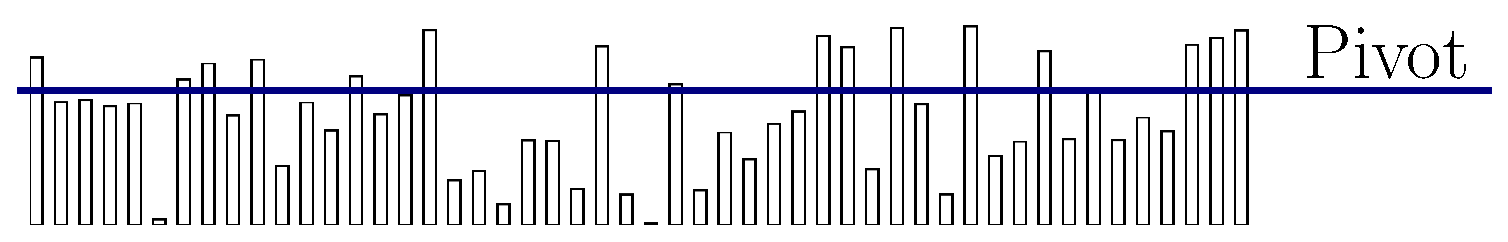
\includegraphics[width=\linewidth]{imgs/partitionDefn/partitionDefn1Ann.eps}

%   \vspace{2cm}

%   {\color{blue} An array partitioned relative to the pivot value:}
%   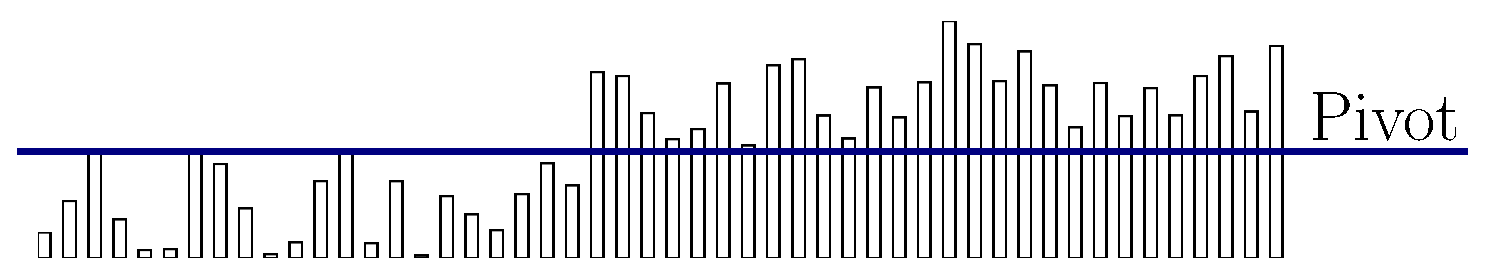
\includegraphics[width=\linewidth]{imgs/partitionDefn/partitionDefn2Ann.eps}
% \end{frame}

\begin{frame}[t]{}
  \begin{figure}
    \begin{center}
      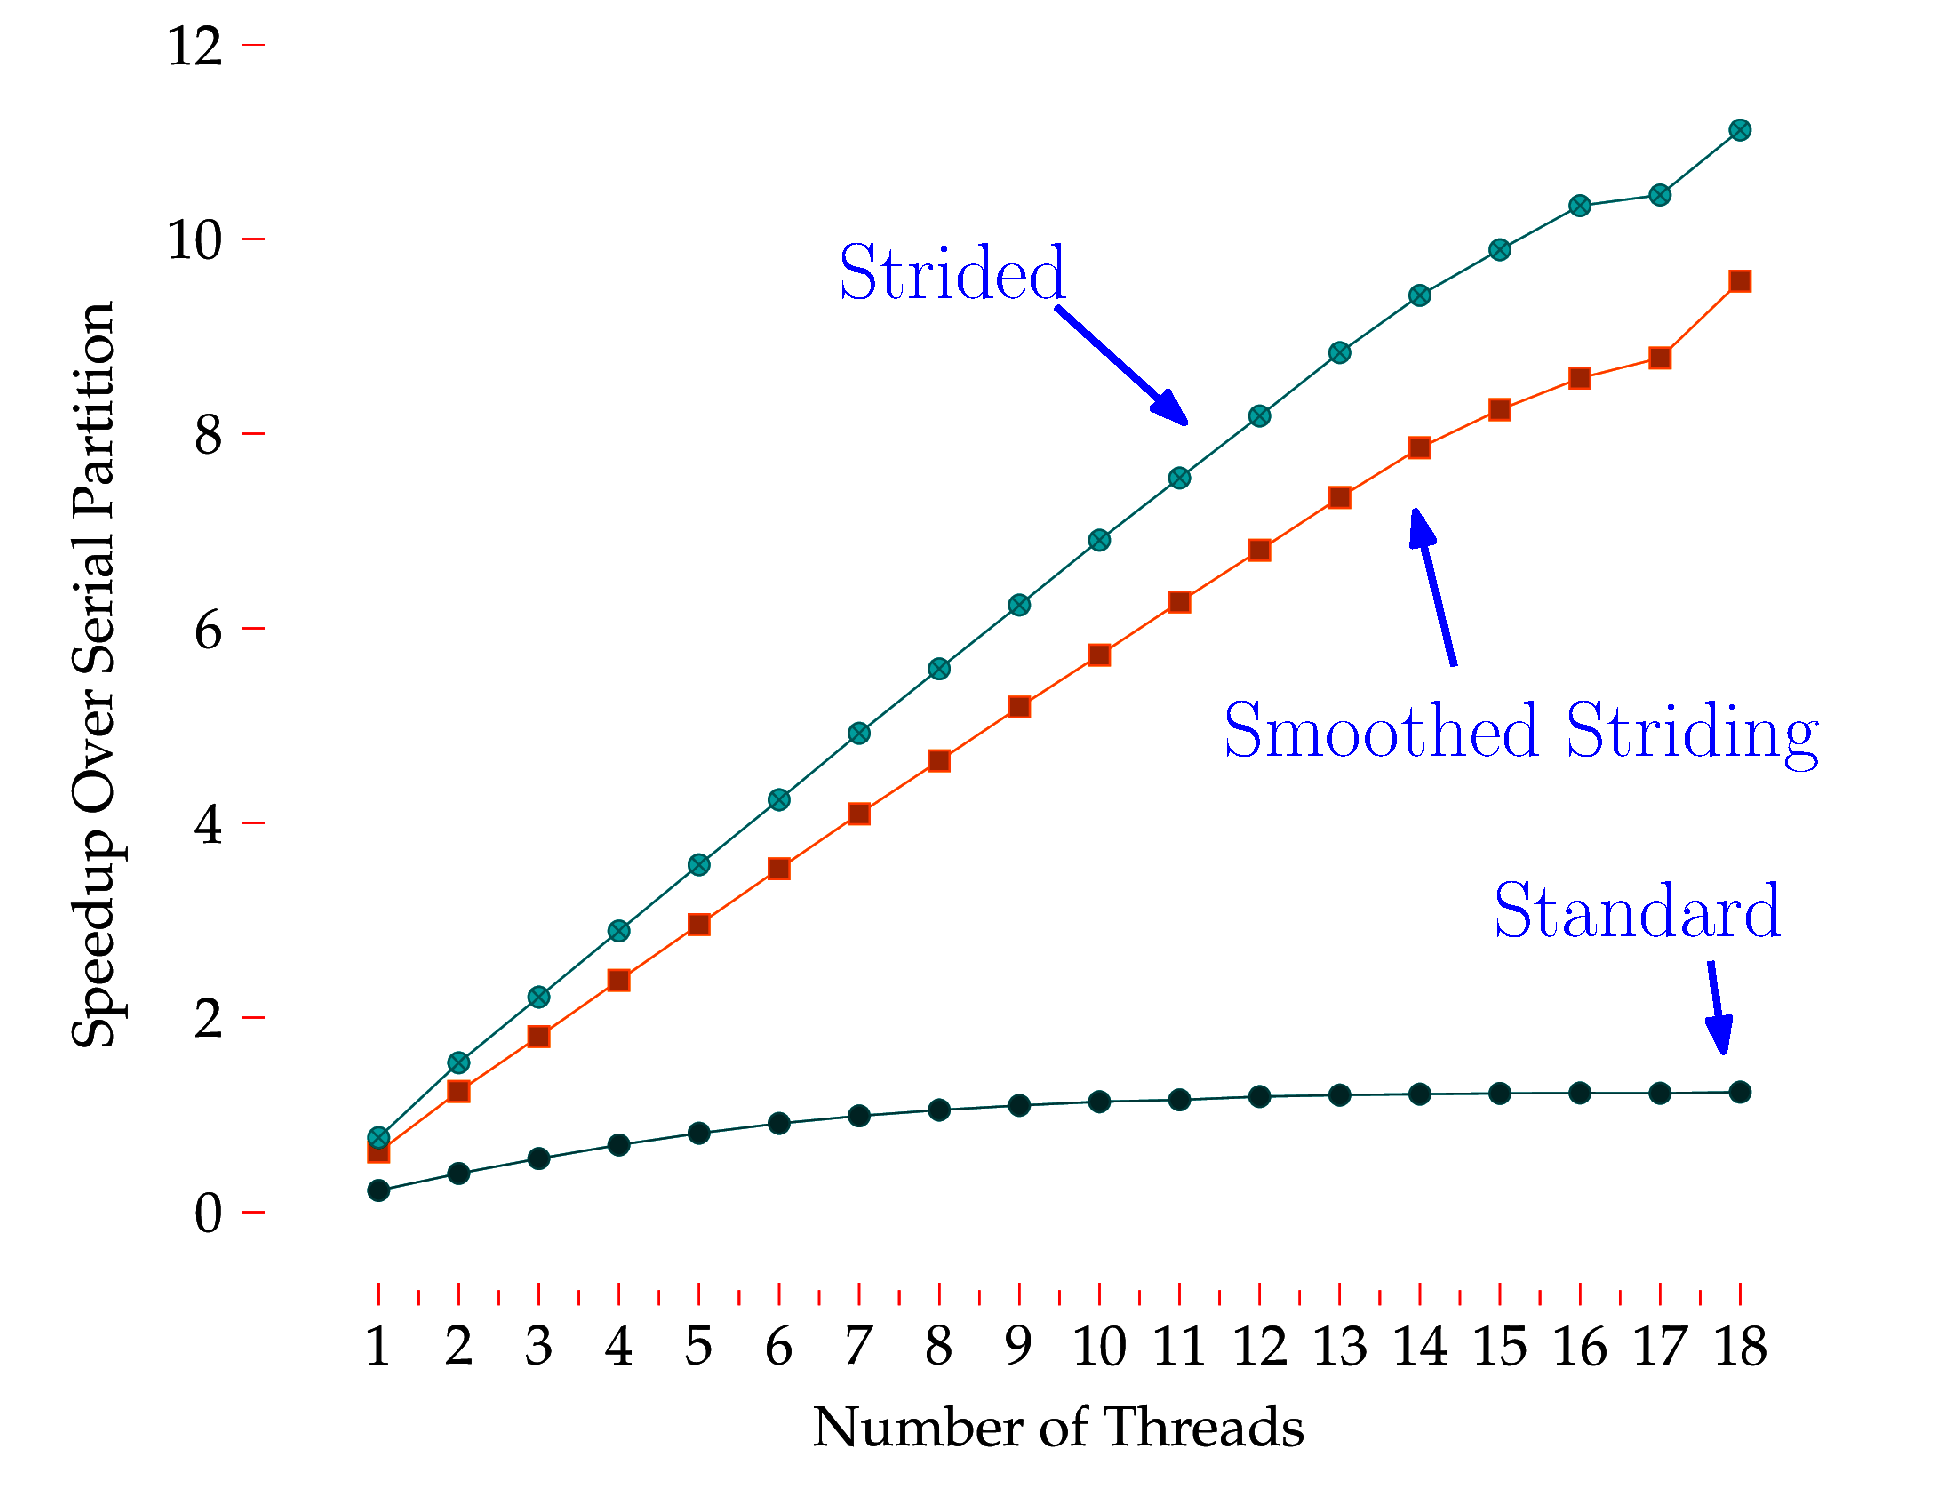
\includegraphics[width=0.9\linewidth]{imgs/compiledGraph.eps}
    \end{center}
  \end{figure}
\end{frame}

\begin{frame}[t]{}
\textbf{Strided Algorithm groups:}
\begin{figure} 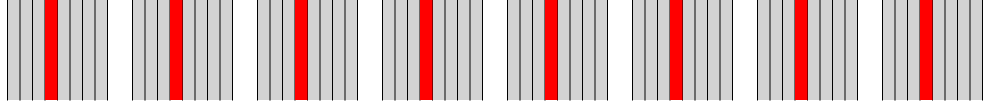
\includegraphics[width=\linewidth]{imgs/stridedAlgHighlighted.png} \end{figure}

\vspace{2cm}

\textbf{Smoothed-Striding Algorithm groups:}
\begin{figure} 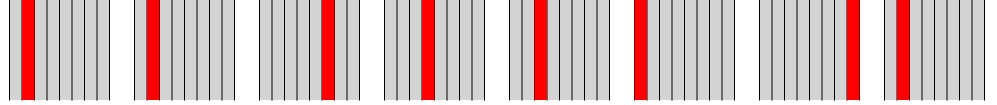
\includegraphics[width=\linewidth]{imgs/smoothedStridingAlgHighlighted.png} \end{figure}
\end{frame}

\begin{frame}[t]{}
  \textbf{Solution:}
  \begin{itemize}
    \item Store a single group
    \item Determine other groups by a circular shift
  \end{itemize}

Note: groups are not independent, but each is random.

\vspace{0.5cm}
\begin{figure} 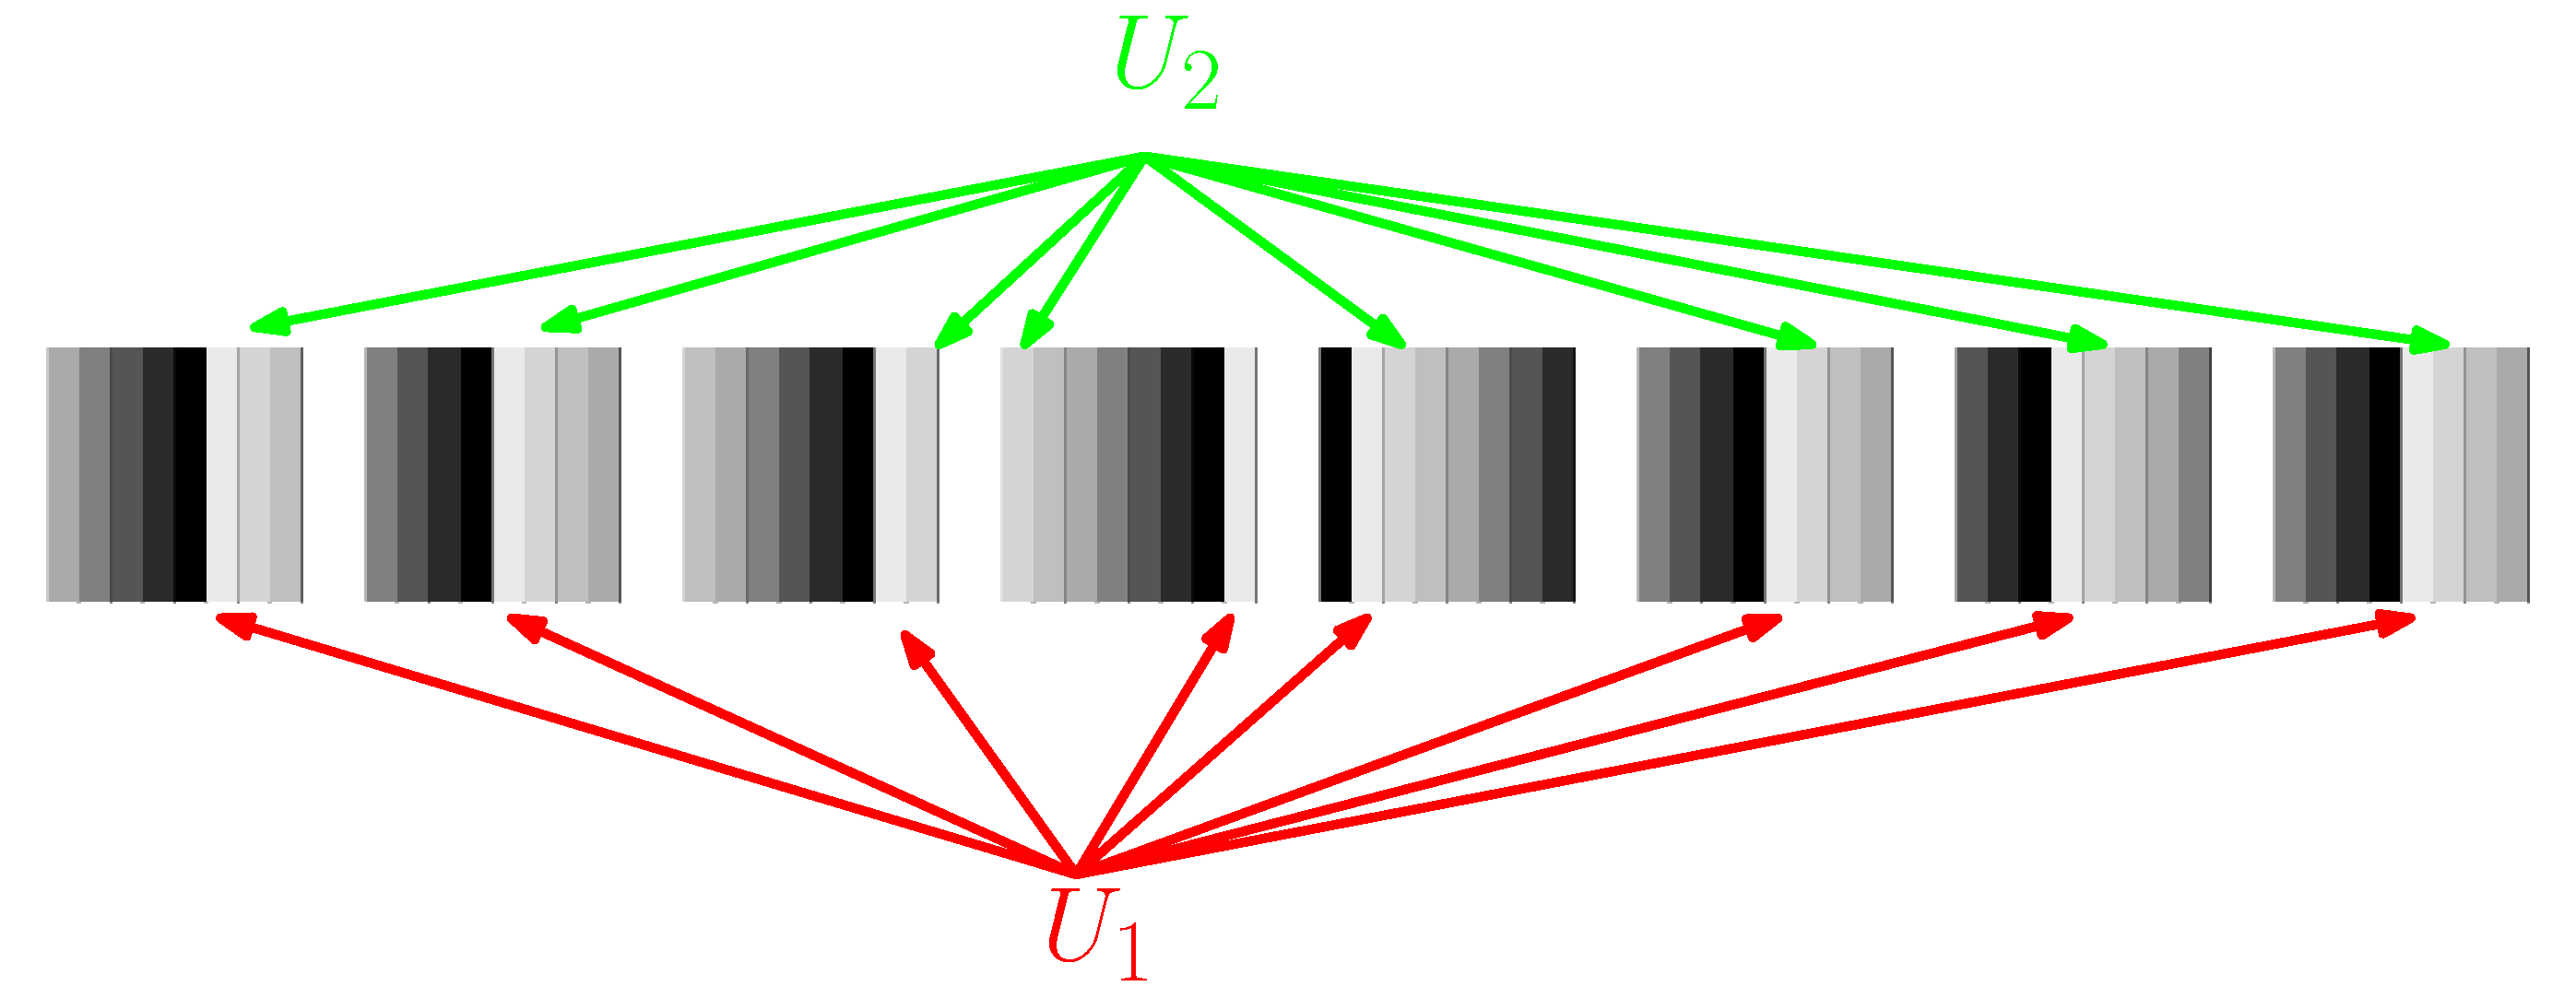
\includegraphics[width=\linewidth]{imgs/blackrainbowAlt.eps} \end{figure}	
\end{frame}

\begin{frame}[t]{Smoothed Striding Algorithm}

  {\color{blue}Form groups $U_i$ containing a random element from
  each chunk.}
  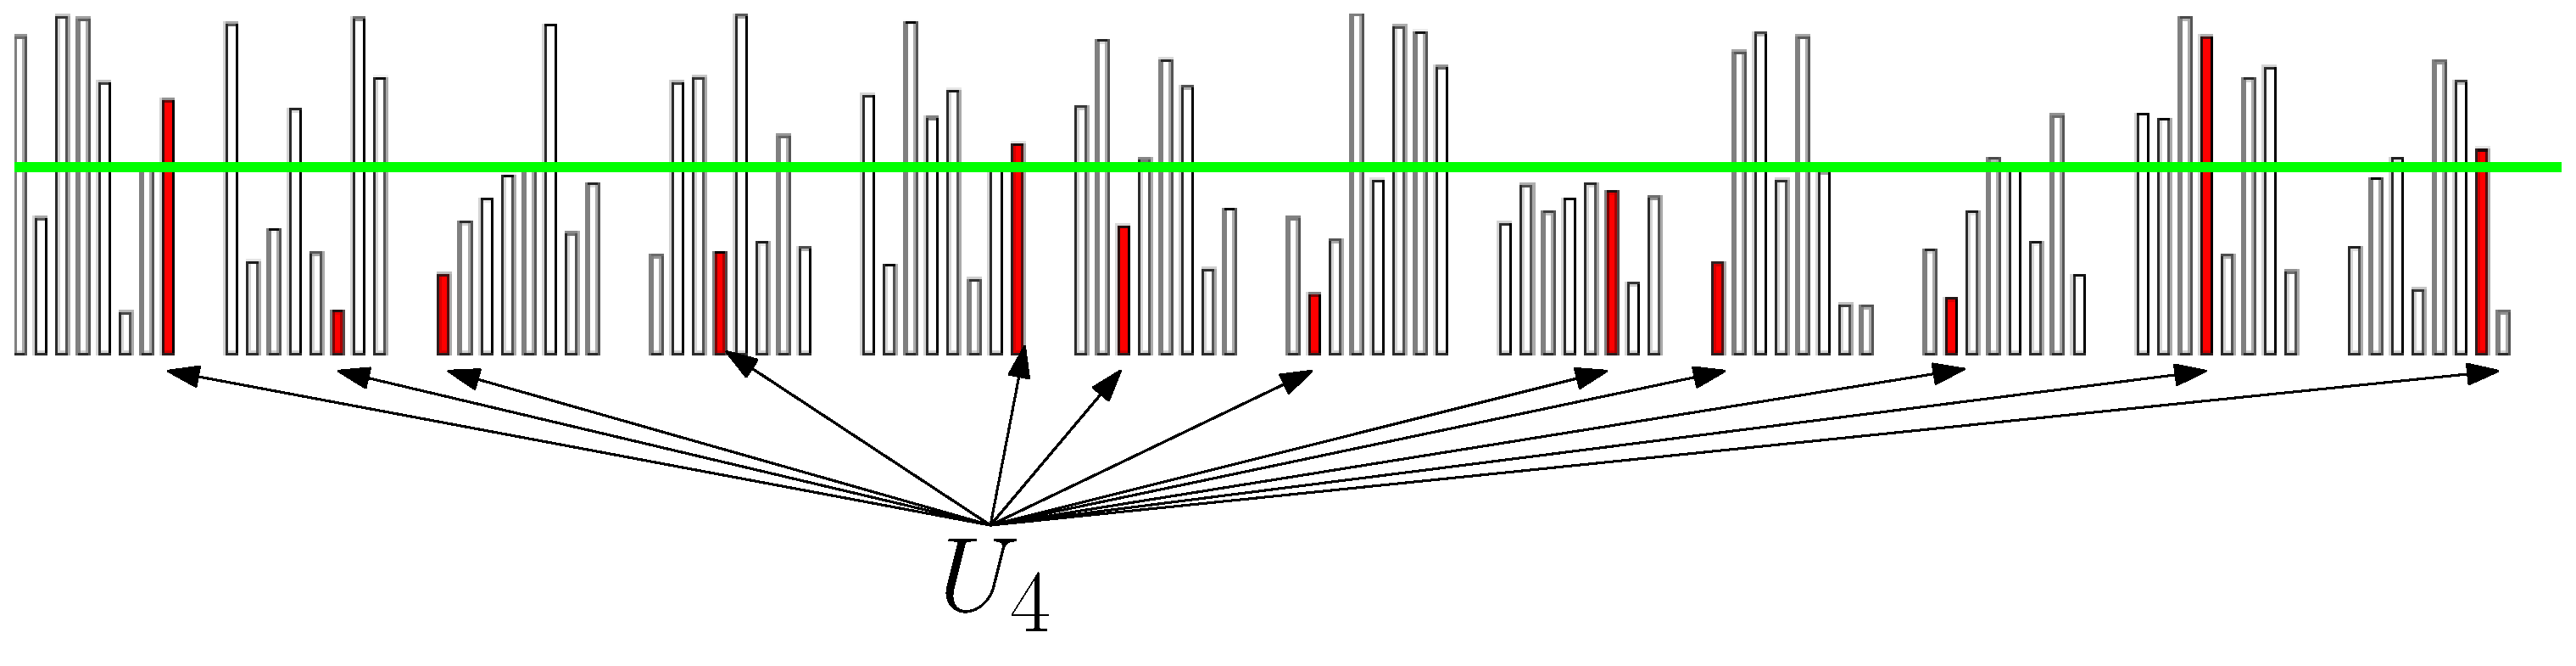
\includegraphics[width=\linewidth]{imgs/smoothedStridingAlgSim/sim2.eps}
  
  \vspace{0.5cm}
  {\color{blue}Perform \textbf{serial partitions} on each $U_i$ \textbf{in parallel over the $U_i$'s}.}
  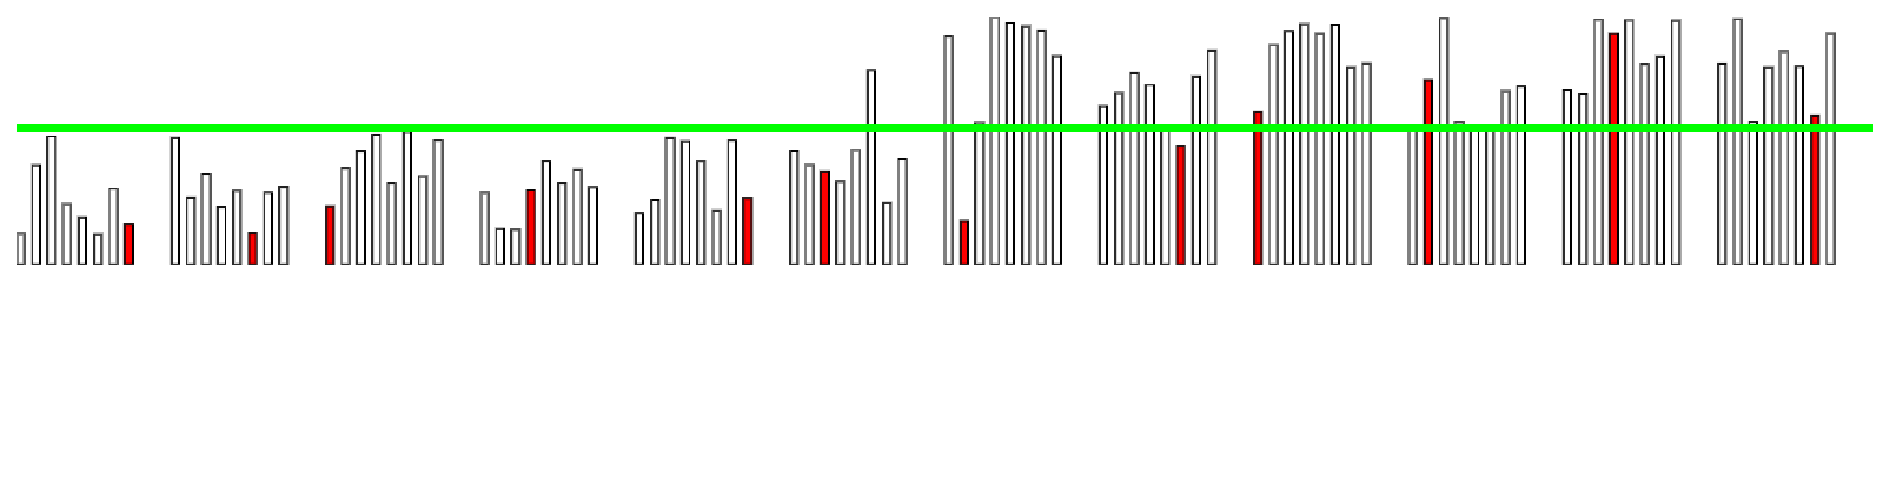
\includegraphics[width=\linewidth]{imgs/smoothedStridingAlgSim/sim3.eps}
\end{frame}

\begin{frame}[t]{Smoothed Striding Algorithm}

  {\color{blue}Partitioning the $U_i$'s ``partially partitions''
the array.}
  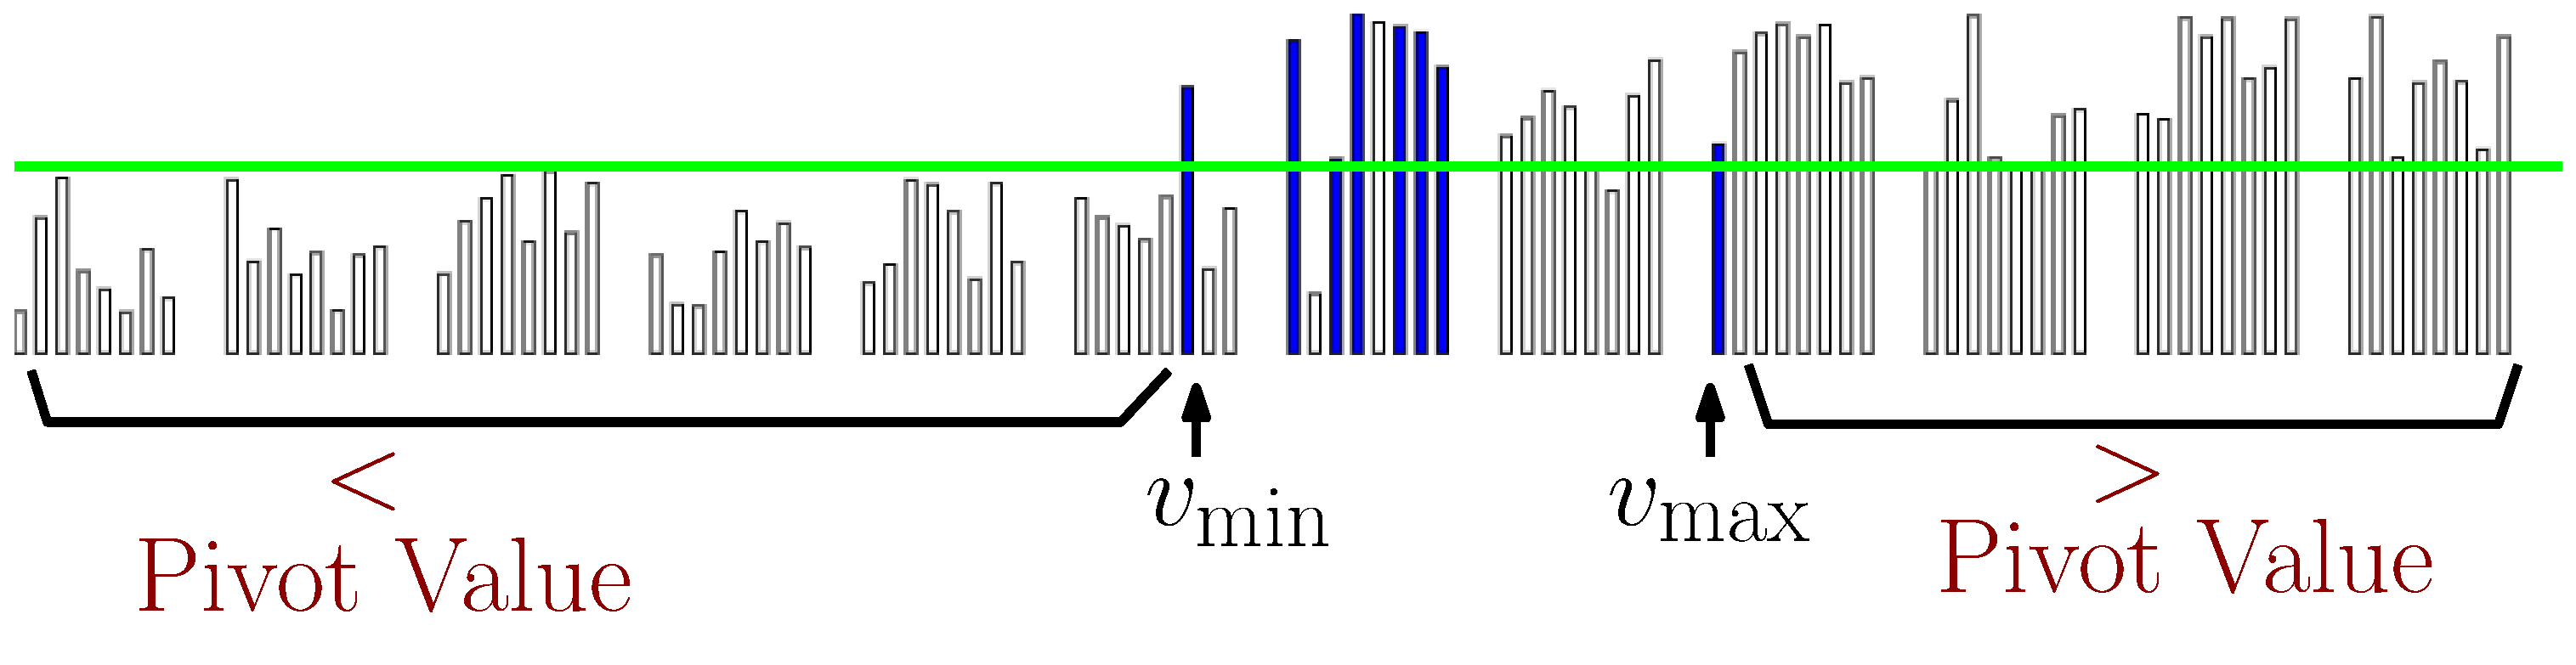
\includegraphics[width=\linewidth]{imgs/smoothedStridingAlgSim/sim4.eps}

  \vspace{0.5cm}
  {\color{blue}Recursively partition the subarray.}
  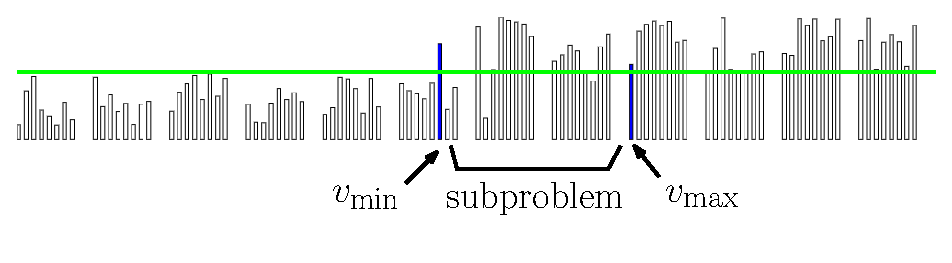
\includegraphics[width=\linewidth]{imgs/smoothedStridingAlgSim/sim45.eps}
\end{frame}

\end{document}
